\chapter{Psalm 36}

\begin{figure}
  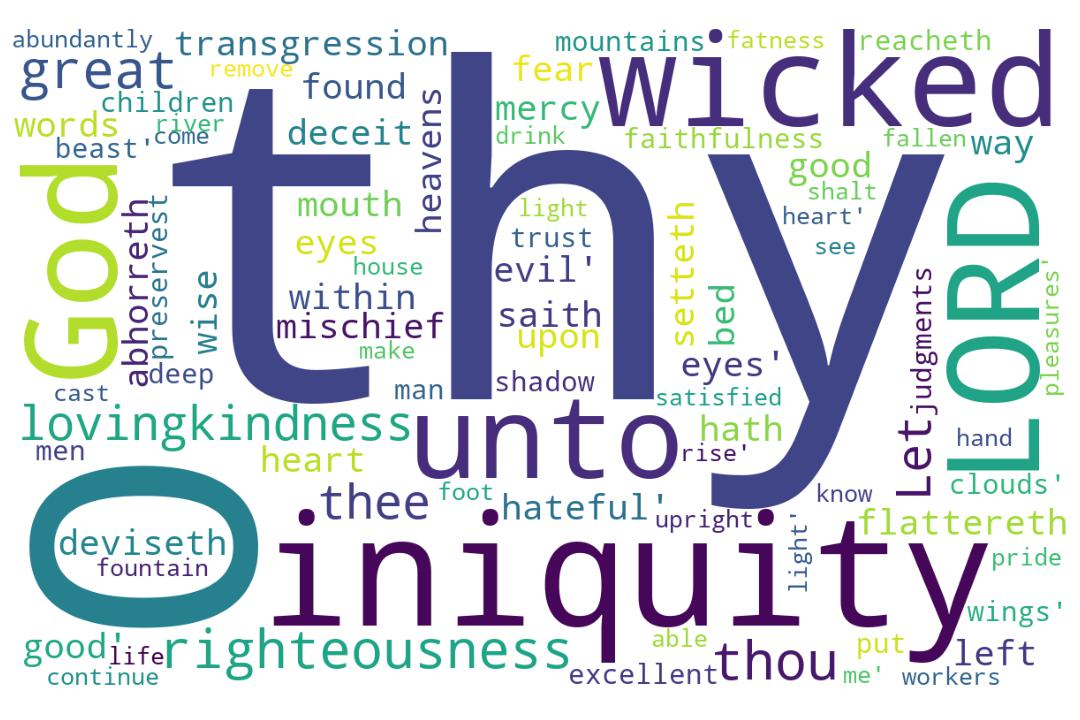
\includegraphics[width=\linewidth]{19OT-Psalms/Psalm36-WordCloud.jpg}
  \caption{Psalm 36 Word Cloud}
  \label{fig:Psalm 36 word Cloud}
\end{figure}
%%%%%%%%%%%%%%%%%%%%%%%%%%%%%%%%%%%%%%%%%
%%%%%%%%%%%%%%%%%%%%%%%%%%%%%%%%%%%%%%%%%

\marginpar{\scriptsize \centering \fcolorbox{bone}{lime}{\textbf{THE WICKED \& THE FAITHFUL}}\\ (Psalm 36:1-12) 
\begin{compactenum}[I.][8]
    \item The Wicked Have No \textbf{No Fear of God} \index[scripture]{Psalms!Psa 036:01} ( Psa 36:01)
    \item The Wicked Practice \textbf{Self Flattery} \index[scripture]{Psalms!Psa 036:02} (Psa 36:2)
    \item The Wicked Miss the \textbf{Faithfulness of God} \index[scripture]{Psalms!Psa 036:05} (Psa 36:05)
    \item The Faithful Partake of the \textbf{Fatness of God's House} \index[scripture]{Psalms!Psa 036:08} (Psa 36:08)
    \item The Faithful Partake of the \textbf{Fountain of Life} \index[scripture]{Psalms!Psa 036:09} (Psa 36:09)
    \item The Faithful are Delivered from the \textbf{Foot of Pride} and the Hand of the Wicked \index[scripture]{Psalms!Psa 036:11} (Psa 36:11)
    \item The Wicked will \textbf{Fall and Not Rise} \index[scripture]{Psalms!Psa 036:12} (Psa 36:12)
\end{compactenum} }

\marginpar{\scriptsize \centering \fcolorbox{bone}{yellow}{\textbf{THE WICKED \& THE RIGHTEOUS}}\\ (Psalm 36:1-12) 
\begin{compactenum}[I.][8]
    \item \textbf{Direction} of the Wicked \index[scripture]{Psalms!Psa 036:02} (Psa 36:2)
    \item \textbf{Deceit} of the Wicked \index[scripture]{Psalms!Psa 036:03} (Psa 36:3)
    \item \textbf{Devices} of the Wicked \index[scripture]{Psalms!Psa 036:04} (Psa 36:4)
    \item \textbf{Distinction} of the Righteous \index[scripture]{Psalms!Psa 036:05}\index[scripture]{Psalms!Psa 036:06} (Psa 36:5, 6)
    \item \textbf{Decision} of the Righteous \index[scripture]{Psalms!Psa 036:07}\index[scripture]{Psalms!Psa 036:08}\index[scripture]{Psalms!Psa 036:09} (Psa 36:7, 8, 9)
    \item \textbf{Deliverance} of the Righteous \index[scripture]{Psalms!Psa 036:10} (Psa 36:10)
    \item \textbf{Deeds} of the Wicked \index[scripture]{Psalms!Psa 036:12} (Psa 36:12)
    \item \textbf{Destination} of the Wicked \index[scripture]{Psalms!Psa 036:12} (Psa 36:12)
\end{compactenum} }

\marginpar{\scriptsize \centering \fcolorbox{bone}{black}{\textcolor{white}{\textbf{7 SINS OF THE WICKED}}}\\ (Psalm 36:1-12) 
\begin{compactenum}[I.][8]
    \item Has no \textbf{Fear of God} \index[scripture]{Psalms!Psa 036:01} (Psa 36:1)
    \item Exercises \textbf{Self-flattery} \index[scripture]{Psalms!Psa 036:02} (Psa 36:2)
    \item Chooses \textbf{Iniquity}  \index[scripture]{Psalms!Psa 036:02} \index[scripture]{Psalms!Psa 036:03} (Psa 36:2, 3)
    \item Practice \textbf{Deceit} \index[scripture]{Psalms!Psa 036:03} (Psa 36:3)
    \item Rejects \textbf{Wisdom} \index[scripture]{Psalms!Psa 036:03} (Psa 36:3)
    \item Pursues \textbf{Mischief} \index[scripture]{Psalms!Psa 036:04} (Psa 36:4)
    \item Does not \textbf{Abhor Evil} \index[scripture]{Psalms!Psa 036:05} (Psa 36:5)
\end{compactenum} }

\footnote{\textcolor[cmyk]{0.99998,1,0,0}{\hyperlink{TOC}{Return to end of Table of Contents.}}}\footnote{\href{https://audiobible.com/bible}{\textcolor[cmyk]{0.99998,1,0,0}{Psalms Audio}}}\textcolor[cmyk]{0.99998,1,0,0}{To the chief Musician, \emph{A Psalm} of David the servant of the LORD.}\\
\\
\textcolor[cmyk]{0.99998,1,0,0}{The \fcolorbox{bone}{MYGOLD}{transgression} of the wicked saith within my heart, \emph{that} \emph{there} \emph{is} \fcolorbox{bone}{lime}{no fear} of God before his eyes.}
[2] \textcolor[cmyk]{0.99998,1,0,0}{For he \fcolorbox{bone}{lime}{flattereth} himself in his own eyes, until his iniquity be found to be hateful.}
[3] \textcolor[cmyk]{0.99998,1,0,0}{The words of his mouth \emph{are} iniquity and deceit: he hath left off to be wise, \emph{and} to do good.}
[4] \textcolor[cmyk]{0.99998,1,0,0}{He deviseth mischief upon his bed; he setteth himself in a way \emph{that} \emph{is} not good; he abhorreth not evil.}
[5] \textcolor[cmyk]{0.99998,1,0,0}{Thy mercy, O LORD, \emph{is} in the heavens; \emph{and} thy \fcolorbox{bone}{lime}{faithfulness} \emph{reacheth} unto the clouds.}
[6] \textcolor[cmyk]{0.99998,1,0,0}{Thy \fcolorbox{bone}{MYGOLD}{righteousness} \emph{is} like the great mountains; thy judgments \emph{are} a great deep: O LORD, thou preservest man and beast.}
[7] \textcolor[cmyk]{0.99998,1,0,0}{How excellent \emph{is} thy lovingkindness, O God! therefore the children of men put their trust under the shadow of thy wings.}
[8] \textcolor[cmyk]{0.99998,1,0,0}{They shall be abundantly satisfied with the \fcolorbox{bone}{lime}{fatness} of thy house; and thou shalt make them drink of the river of thy pleasures.}
[9] \textcolor[cmyk]{0.99998,1,0,0}{For with thee \emph{is} the \fcolorbox{bone}{lime}{fountain} of life: in thy light shall we see light.}\footnote{\textbf{Proverb 13:14} - The law of the wise is a fountain of life, to depart from the snares of death.}\footnote{\textbf{Proverb 14:27} - The fear of the LORD is a fountain of life, to depart from the snares of death.}
[10] \textcolor[cmyk]{0.99998,1,0,0}{O continue thy lovingkindness unto them that know thee; and thy \fcolorbox{bone}{MYGOLD}{righteousness} to the upright in heart.}
[11] \textcolor[cmyk]{0.99998,1,0,0}{Let not the \fcolorbox{bone}{lime}{foot} of pride come against me, and let not the hand of the wicked remove me.}
[12] \textcolor[cmyk]{0.99998,1,0,0}{There are the workers of iniquity \fcolorbox{bone}{lime}{fallen}: they are cast down, and shall not be able to rise.}



